\documentclass[onecolumn, draftclsnofoot,10pt, compsoc]{IEEEtran}
\usepackage{graphicx}
\usepackage{url}
\usepackage{setspace}
\usepackage{multirow}

\usepackage{geometry}
\geometry{textheight=9.5in, textwidth=7in}

% 1. Fill in these details
\def \CapstoneTeamName{		Capstone 41}
\def \CapstoneTeamNumber{		41}
\def \GroupMemberOne{			David Corbelli}
\def \GroupMemberTwo{			Jason Ye}
\def \GroupMemberThree{			Zixuan Feng}
\def \CapstoneProjectName{		Website and Application for Health Careers in Oregon}
\def \CapstoneSponsorCompany{	Oregon Department of Education}
\def \CapstoneSponsorPerson{		Art Witkowski}

% 2. Uncomment the appropriate line below so that the document type works
\def \DocType{	%Problem Statement
				%Requirements Document
				%Technology Review
				%Design Document
				Spring Progress Report
				}
			
\newcommand{\NameSigPair}[1]{\par
\makebox[2.75in][r]{#1} \hfil 	\makebox[3.25in]{\makebox[2.25in]{\hrulefill} \hfill		\makebox[.75in]{\hrulefill}}
\par\vspace{-12pt} \textit{\tiny\noindent
\makebox[2.75in]{} \hfil		\makebox[3.25in]{\makebox[2.25in][r]{Signature} \hfill	\makebox[.75in][r]{Date}}}}
% 3. If the document is not to be signed, uncomment the RENEWcommand below
%\renewcommand{\NameSigPair}[1]{#1}

%%%%%%%%%%%%%%%%%%%%%%%%%%%%%%%%%%%%%%%
\begin{document}
\begin{titlepage}
    \pagenumbering{gobble}
    \begin{singlespace}
    	
\includegraphics[height=4cm]{coe_v_spot1}
        \hfill 
        % 4. If you have a logo, use this includegraphics command to put it on the coversheet.
        %\includegraphics[height=4cm]{CompanyLogo}   
        \par\vspace{.2in}
        \centering
        \scshape{
            \huge CS Capstone \DocType \par
           	\huge [cs462 Sp17] \par
            {\large\today}\par
            \vspace{.5in}
            \textbf{\Huge\CapstoneProjectName}\par
            \vspace{.5in}
           
            {\large Prepared by }\par
           
            % 5. comment out the line below this one if you do not wish to name your team
   
            \vspace{5pt}
            \textbf{\Huge\ \CapstoneTeamName}\par
            }
            \vspace{60pt}
        
        \begin{abstract}
        % 6. Fill in your abstract    
The application and website for Oregon Health Science Careers is a guide for middle school and high school level students to learn about health science careers.  
Between an application and website, the service shall provide information as exploration tool for students looking for future careers in health science. 
Due to the many fields under the classification of health and science, it may be difficult for a student beginning to take an interest in the subject to find the proper path they’re looking for. 
As a development team we will focus on developing an exploratory website and then develop corresponding applications for two major platforms, Android and iOS.
Through our platform, students will explore pathways and careers in health and science. 
In this paper, we will discuss our design and specifications of the applications and website we plan to develop. 
        \end{abstract} 
        
    \end{singlespace}
\end{titlepage}
\newpage
\pagenumbering{arabic}
\tableofcontents
% 7. uncomment this (if applicable). Consider adding a page break.
%\listoffigures
%\listoftables
\clearpage

% 8. now you write!
\section{Introduction}

\noindent Our project was commissioned by Art Witkowski, an educational specialist from the Oregon Department of Education. The problem we were faced with was easing the difficulty middle school and high school students face when trying to learn about careers in health sciences. 
The solution our client proposed was for our group to develop a website and application for students, their families, and advisors to use as a learning exploration tool. 
The information present on this site, given to us by the Department of Education, provides information specific to each career path, including available job opportunities and supporting schools and universities. 
\\ 

\noindent Our project specifications require the development of our website and application in such a way that users are able to navigate through pages containing information on various career paths.
Along with our technology implementation requirements from our technology review document, we have also listed several assumptions and dependencies for which we would rely upon our client. These dependencies include: information concerning health science careers provided by the Oregon Department of Education,  web and database hosting solutions for our final product, also to be provided by the Oregon Department of Education, and thirdly, the publishing of our developed mobile application the be handled by the Oregon Department of Education.
\\ 

\noindent Our initial goals for this assignment in-line with creating a health careers website and application include the implementation of a relational database utilizing MySQL, the Bootstrap styling framework for visual appearance, templated page generation for efficiency and ease of use, Google Analytics for site traffic monitoring, user testing for feedback, and a hybrid Android application developed using the Android Studio software development kit.
\\

\begin{figure}[h]
\centerline{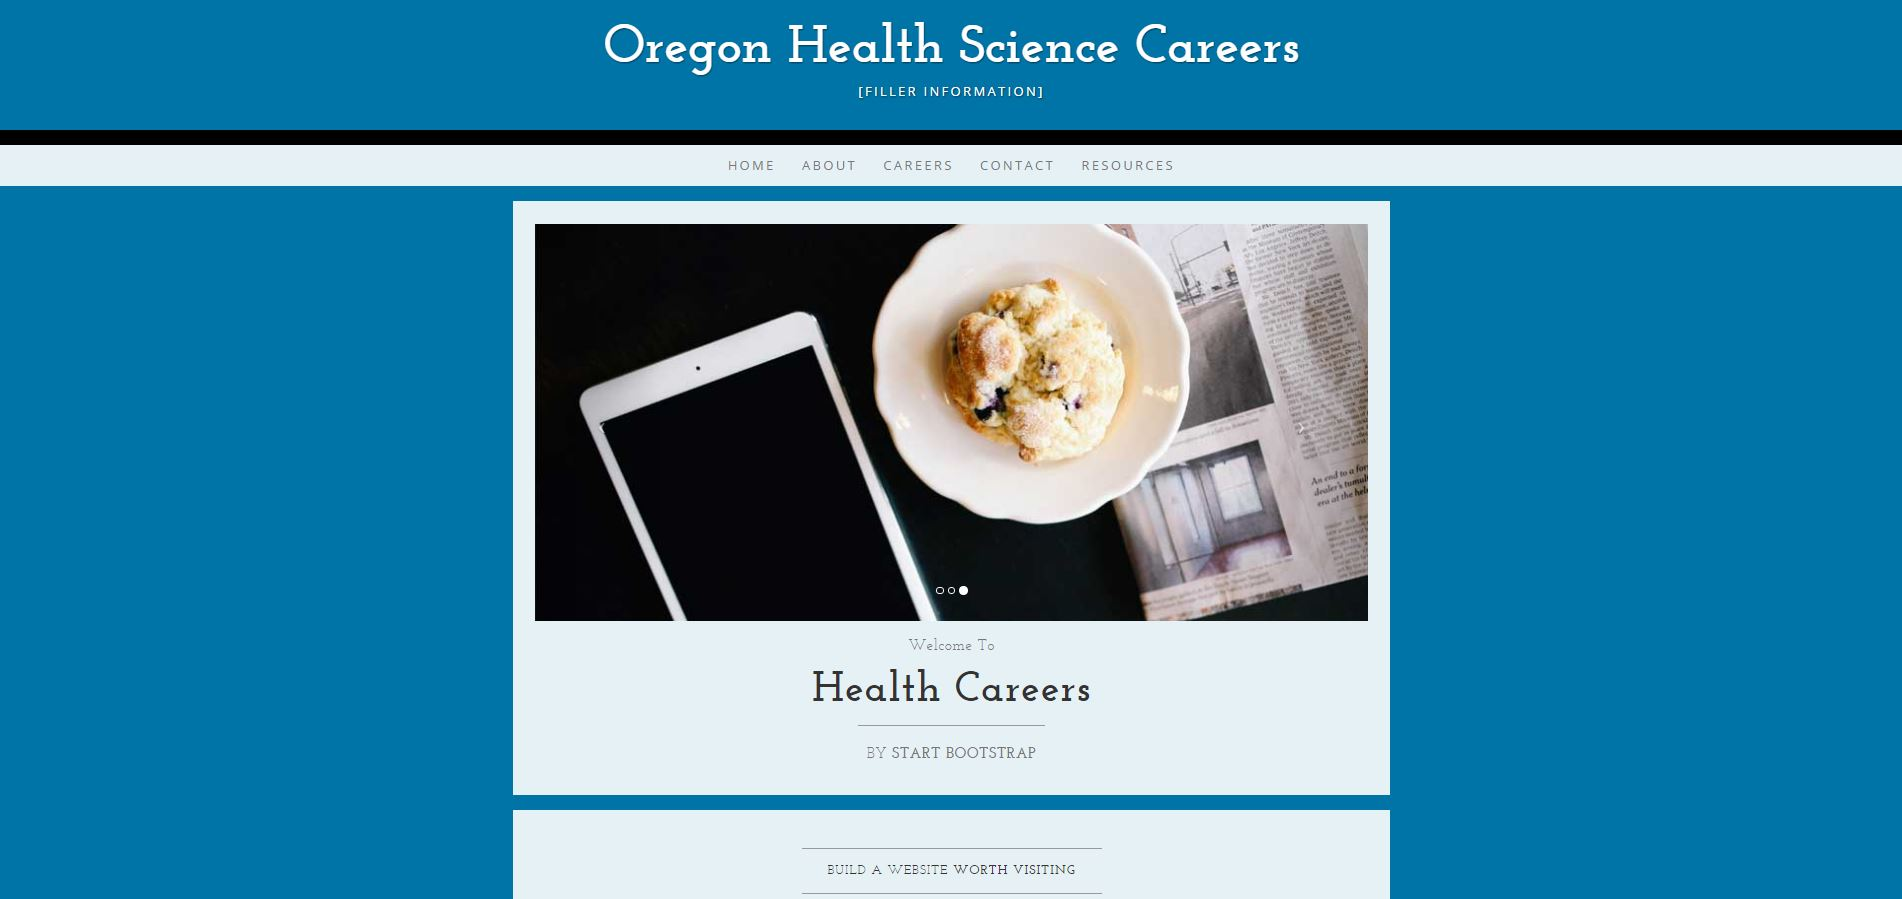
\includegraphics[scale=.3]{Figure_1.jpg} }
\caption{An early version of our desktop site homepage}
\end{figure}

\noindent Once our we had progressed in our development, beyond our requirements we were able to implement several stretch-goal features. For convenience, we have begun to implement a CSV upload system for adding to or updating information within our database.
This will allow our client to manage certain features of our site without having to learn the phpMyAdmin interface. We were also able to add an email contact feature allowing users to send contact messages to an email address to be specified by our client.
By including this feature directly on the website, we hope users will be more inclined to interact with our site and seek additional information if questions should arise.


\section{Progress To-Date}

\subsection{Desktop Website}

\noindent The first component we worked to complete was our desktop website. Our initial design was based on a found template utilizing bootstrap. We have since taken steps towards changing the color scheme and of the design of the website and have added functionality necessary to our project. We have converted most of the files from HTML to PHP files containing HTML components; this allows us to run server-side scripting previously unavailable in earlier formats. We were able to develop a template for our career information pages that display information pulled from our MySQL database using PHP scripting. we were also able to include an email submission form on our contact page and a sortable index for our career paths. The majority of our HTML pages are left with lorem ipsum filler text as our client was never able to send us the display information he desired. This information can be easily swapped out through editing the HTML files and we will cover this in our usage guide for our client. 

\begin{figure}[h]
\centerline{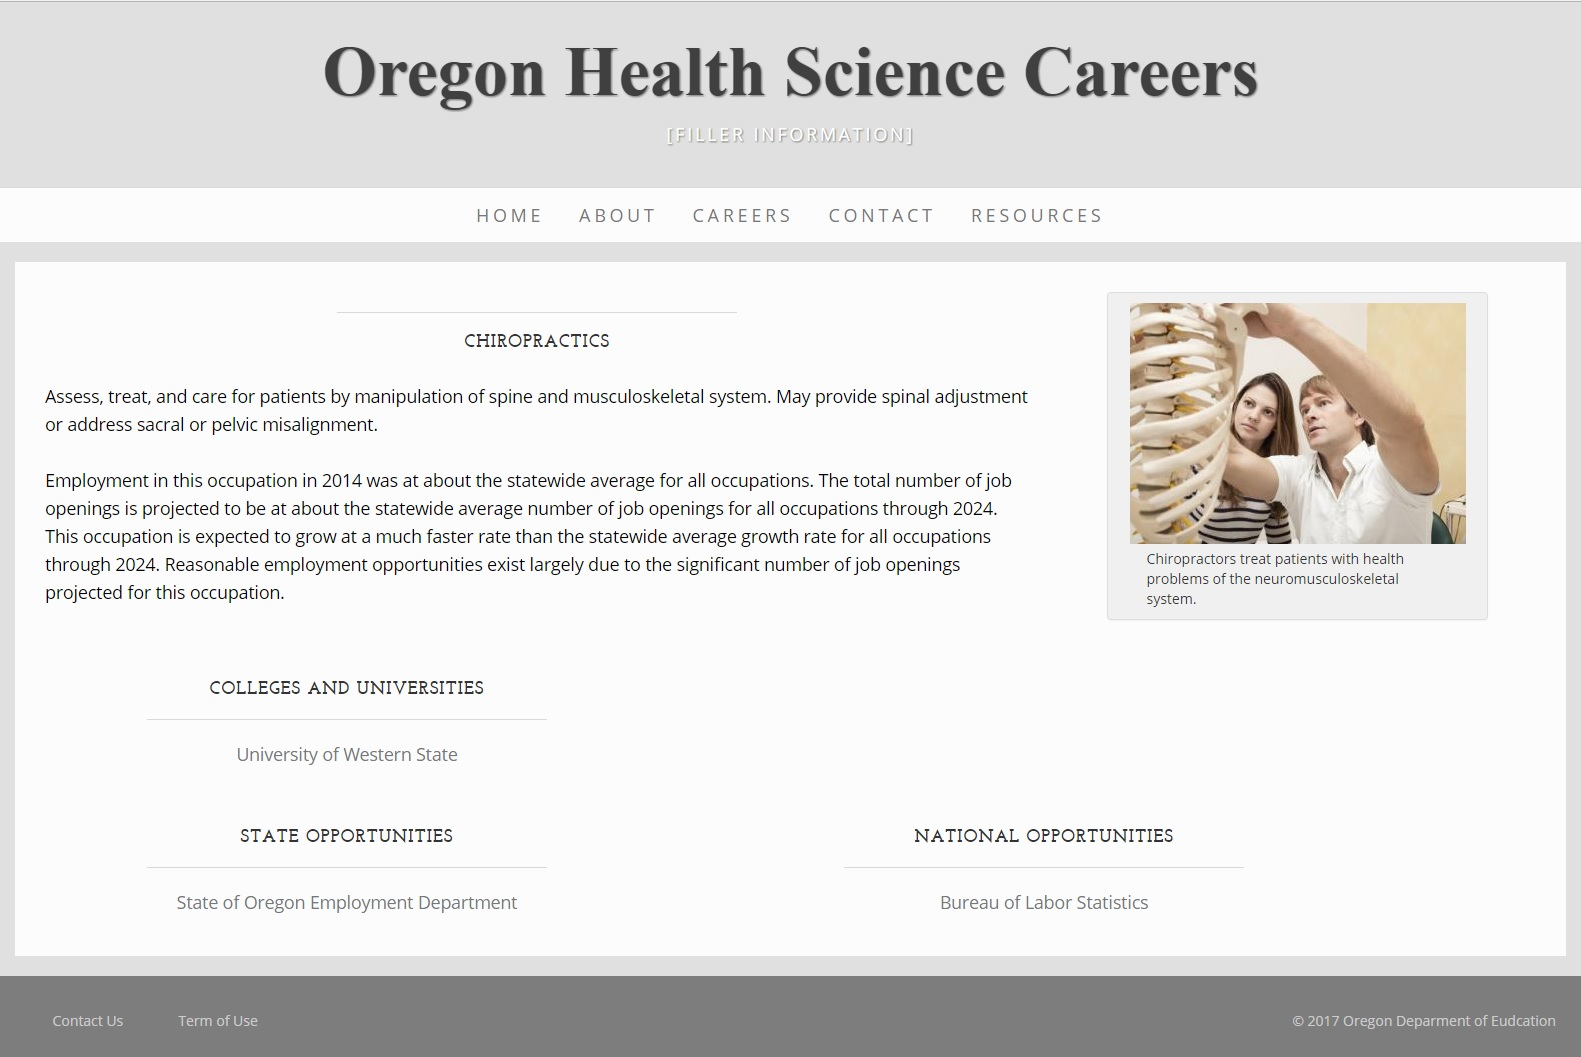
\includegraphics[scale=.3]{Figure_2.jpg} }
\caption{The current appearance of our Chiropractics information page}
\end{figure}

\subsection{Mobile Application}

\noindent As for Mobile application, we finished the “Oregon health Careers Path “mobile app in Android platform. At first of our project, we contacted with client to ask the mobile application requirements, we reached the agreement to design a mobile application in android platform. There are three reasons: first, android is open source operation system with quantity users. Secondly, android platform could offer technology framework in various android community. Because “Oregon Health Careers Path” is focusing on education materials, and android platform could provide updating content and expansions, it is very important for future administer to notify visitor about updates and maintenances. Compared with IOS, Android could help client have a better maintenance and manage environment. What is more, android application is easy to learn and adopt, the majority language is JAVA, which is an objective-oriented language we could operate data and collect data from users and show up on the screen. 
Due to the development, originally we chose three different tools to develop the android application, Android Studios, Corona and Appcelerator Titanium. After comparison, we chose the Android Studios, the reasons are android studio has the reconstruction of the exclusive and quick fixes, and the tip could hint and help us for usability and compatibility. And the various functions of Android Studio could combine the coding and Interface together, and it could also off the C++ implement, which give us an easier way to debugging. What is more, the android studio could also provide a emulator which is same as the real device. With using emulator to test, it is effective for us to test our application. \\

\begin{figure}
\centerline{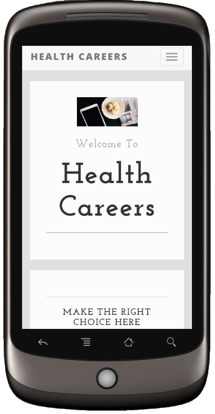
\includegraphics[scale=1.5]{phone.png} }
\caption{The Mobile application}
\end{figure}

\begin{figure}
\centerline{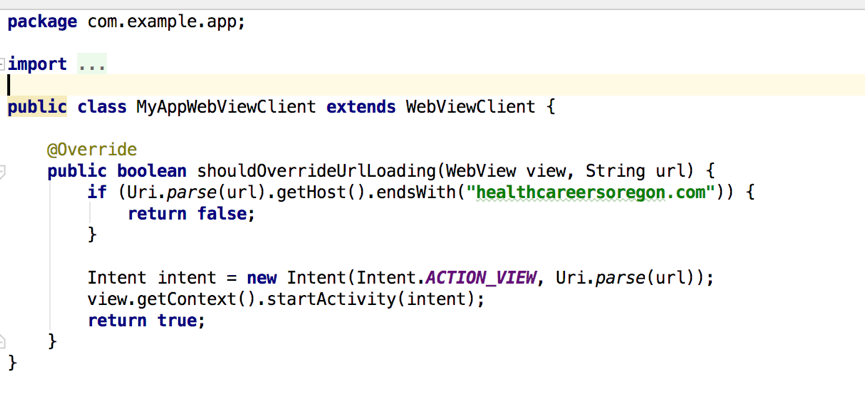
\includegraphics[scale=1]{coding.png} }
\caption{Android Studio Program development}
\end{figure}

\noindent After a almost two month, we developed our mobile application. Within a lot research, we used a Android application template, based on this template, we nest our website in the application. \\

\noindent When we developed the application, we faced a problem, the website interface will not fit with our application, especially for different brand and screens of android devices. Firstly, we tried to fix the interface through JAVA coding, but we still did not fix the problem. Some devices still cannot work for “career list” page. Within a week, we were working on the interface problem of our application. We found we could use our bootstrap template, and the template has a mobile CSS part could allow us to develop the mobile interface. And this CSS will tell the screen automatically and adjust all the CSS coding. 
After fixing the interface problem, we finished the mobile application, and it has all the functionality we designed. We found users to test our applications, there is not issues found. All in all, the mobile application we finished correctly and successfully, we meet all the requirement provided by our client.  \\

\subsection{Database Setup}
\noindent For the database setup, we have acquired the necessary sources for accessing the database owned by the Oregon State University server. 
The server is only limited to students who are engineering major. 
Thus, permission to accessibility must be given by the engineering department. 
In order to gain access to the server, the username and password were given by the university administrator. 
After receiving the necessary information, we could log in to the server by using the phpMyAdmin, a software tool that handle the administration of MySQL over the Web, to host the database. 
This software supports a wide range of frequently used operations on MySQL such as managing database, tables, columns, relations, indexes, users, permission and more. 
This performance can be done by through user interface and directly execute any SQL statement.\\

\noindent In addition to using the phpMyAdmin, it is highly supportive on MySQL database. 
We have chosen to operate with MySQL database because it offers the most beneficial functions. 
MySQL database provide us to adjust, manage, and optimize easily when working with large data sets.
By connecting and accessing to the MySQL database using the school client, we simply started implementing tables and relational schemas.\\ 

\noindent After successfully accessing the MySQL database, I have the ability to handle essential features provide by the database. 
With the information given by our client, I have broken down the data into multiple relational tables: Careers, CareerLink, Opportunity, and Schools. 
Each table has a primary and foreign keys which are relates to other tables. With these relational tables, the data can be adjusted and managed by using SQL query. 
By using SQL query, the database is enforced with cascading actions of updating, inserting, and deleting data as long as each table has the appropriate primary and foreign keys. 

\subsection{Web Statistics}
\noindent For the purpose of maintaining the website, I have implemented a technology that will analyze the website statistics for trends and success level.
It is a visualization tool kit that can display meaningful data for our client to see. 
This essential tool kit measures the behavior of visitors, track details, and qualifies aspect of the website.\\ 

\noindent To make sure the website is being used in the most efficient and effective way, I have applied web statistic software from Google called the Google Analytics. 
Google analytics offer the best features that benefit our website and mobile application. 
To get the most benefit out of the software, I used the tracking code provided by the software and implemented it into every health science career web pages. 
The purpose of the code is to track data on the site so I can collect data in the analytics property. Thus, I can analyze user interaction and activity when a certain web page is being clicked on. 
After implementing the tracking code, varieties of data are shown on the software. 
These data can be used for analysis and optimization for future purposes.\\

\begin{figure}[h]
\centerline{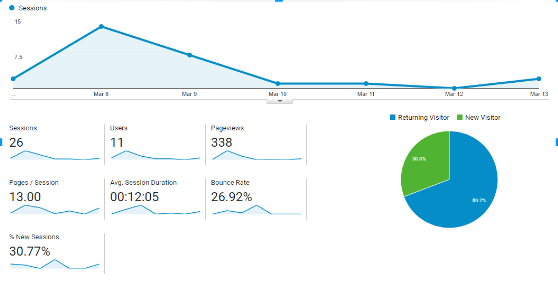
\includegraphics[scale=1]{Figure_6.PNG} }
\caption{Google Analytics}
\end{figure}

\subsection{CSV Implementation}
\noindent One of the most important features of our project is to give our client the ability to upload data without accessing the MySQL database. 
A functional program that user could insert a large amount of data by using a file that stores tabular data in plain text. 
The best solution is to provide an Excel sheet as an implementation tool for uploading data into the database.
Thus, most Excel sheet is being used for storing informative, statistical or financial information.
For implementation, I have made several web pages where user could simply upload a comma-separated values (CSV) file with tabular data in plain text. 
The web pages are run in PHP file which programmed in SQL queries and object-oriented language.\\ 

\begin{figure}[h]
\centerline{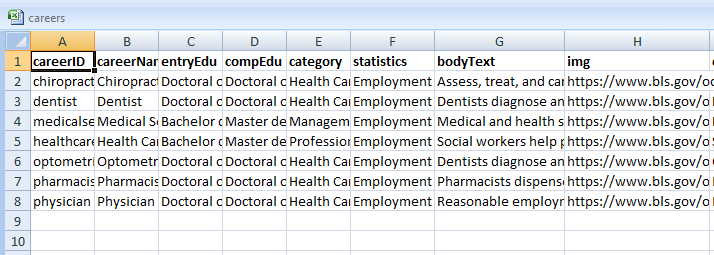
\includegraphics[scale=0.9]{Figure_4.PNG} }
\caption{Excel Sheet with Data}
\end{figure}

\noindent After the user have chosen a valid CSV file and uploaded the file, the program opens the uploaded CSV file with the read only mode and parses data from the file line by line.
This way, the user can verify the data inputs for validation purposes. 
In addition, the program checks for duplication and invalid input from the user to make sure the data are imported correctly.
If the requirements are not met, then a warning message would be in display.\\ 


\section{Remaining Development}

\noindent At our current state we have finished the majority of our functional components; the only remaining implementations are certain bug fixes to be handled in our career deletion CSV upload page and our documentation of our website and application's usage. We have attempted to contact our client so that we may setup the final database hosting solution, but we have yet to receive an answer after sending a series of emails to him and his reply saying he would look into it. We believe we may not have time to setup the database on our own time, but it is in our project requirements that beyond handing off the necessary files, the hosting solution should come from the Department of Education, our client's end.\\

\noindent As far as the success of implementation for importing and updating data using CSV files, deleting a certain data are still in progression. 
The deletion file is having logical and coding issue which does not affect the main purpose of our project. However, it is a recommended and useful tool for our client to have. 
Due to the lack of time and communication with our client, we have set aside the program in future workload.\\ 

\noindent As a group, we also have need to write a usage guide to our project's implementation. This guide will include screenshots of our coding highlighting necessary information with explanations into what changes will give necessary outputs; this information mainly pertaining to our Bootstrap implementation, the CSV uploading system, database connection variables, and PHP MySQL queries. Other necessary information to be listed will pertain to current login information, Google Analytics usage, phpMyAdmin usage basics, email contact setup, and our Android studio development. After we hand off this information, Art should have the necessary tools to implement any future changes.  

\section{Encountered Obstacles}

\noindent We have faced several obstacles towards the completion of our project. One of the most difficult may have been trying to receive information from our client. Nearing the middle of fall term we had asked our client to begin preparing preliminary career information that we may have a plan for our database implementation. By the end of the term, we had not received any information and it took till the last week of December to receive a single populated row for the Chiropractics career path. Over the duration of winter term, despite asking for desired page content for most all of our webpages, the only information we were able to gather was a spreadsheet containing several more career fields by the last week of the term. No other information as to what information should be displayed on the site: welcome message, about information, contact information, or external links were given despite our requests. As such, our solution to time allocation was to pivot our attention to aspects of the site we could work on without our client's input. The tasks we accomplished in the meantime included the development of our CSV upload pages, mobile application, and email submission form. We were able to use lorem ipsum as filler text while creating space for our client to fill in the information he desires at a later date.  

\section{User Testing Results}

\noindent Besides the implantation, as an ending parts of our project, test plays an significant role in our project. We should do the debugging and testing for all the functionality of website and mobile applications. In the design document, originally we planned to use three different ways to do the test. After comparison we found another testing method called “Cognitive walkthrough testing method”. By using this testing method could not only includes all the testing method we designed, but also could runs better than any other testing method. We assigned different testers for different missions include all the function of website and application. When the tester were trying to finish the mission, tester could rate and grade the process of different missions. By reviewing all the test result of cognitive walkthrough, we could get feedback from either positive and negative suggestions, we could fix the problem by reviewing the feedback. 
We assigned six majority questions, which includes all the functionality of website and mobile application:
\\ \\
\noindent Firstly: we let the user negating away from the home page. All the users could finish the mission easily and smoothly, no big issues or problem founded. 
Secondly, we assigned the tester to navigate to specific careers. Several users found that the need to click on the career name to navigate to the career path screen was slightly less intuitive than had we included the ability to click on the career’s row on the career selection screen. To make things easier for a greater range of viewers one of our stretch developments could be to change this feature.
Thirdly, using the contacting page, and send an email to administrator. All the tester could navigate to contacting page easily, and there is no problem found when user send emails. And administrator could receive the email successfully. 
Fourthly, we asked the user to exploring the hot topic from the main page slides. Users could select the image and navigate to the specific career page, but there was very little information being displayer, but when client could provide more information, we could fix this problem. 
Fifthly, the mission was navigating to main page in any pages. All the tester could navigate back to home page in all other pages. But some testers thought they could return home page by clicking the title header, and we agree with that and this could be a worthwhile for future implement.\\

\noindent For the most part, our testing process consisted of gathering feedback from several users we believe are capable enough to distinguish potential usability problems for a greater range of users. 
We assigned every user a set of tasks to complete and report on whether or not each task was found difficult to complete, whether or not users reach their actions’ intended outcomes, what issues were encountered, and evident solutions to these issues.The most blatant issues our users noticed included broken navigation, and lack of content. Other issues included the inability to navigate back to the home screen via clicking on the page header and visibility of certain components when making selections. We have since reviewed these issues and haven taken steps to remedy these components. 

\section{Conclusion}

\noindent Since the beginning of spring term we have made significant progress towards the development of our health careers project. We were able to meet the requirements listed through our technology review document, complete the development of our desktop site and application, and only have stretch goal implementations remaining. While we are still waiting on certain deliverables from our client we are satisfied with our progress.

\end{document}